\documentclass[11pt]{article}

\usepackage[margin=1in]{geometry}
\usepackage{graphicx}
\usepackage{booktabs}
\usepackage{multirow}
\usepackage{array}
\usepackage{caption}
\usepackage{subcaption}
\usepackage{float}
\usepackage{hyperref}

\hypersetup{
  colorlinks=true,
  linkcolor=blue,
  citecolor=blue,
  urlcolor=blue
}

\title{\textbf{Explainable Machine-Learning Pipeline for Post-Cholecystectomy Syndrome Risk Prediction: A Demonstration Report}}
\author{PCS Study Group}
\date{\today}

\begin{document}
\maketitle

\begin{abstract}
This demo report summarizes an end-to-end analytical workflow for predicting post-cholecystectomy syndrome (PCS) using structured clinical data. It is designed as a compact visual overview of the current project outputs rather than a complete journal manuscript.
\end{abstract}

\section{Background}

Post-cholecystectomy syndrome (PCS) may occur after cholecystectomy and can manifest as abdominal pain, dyspepsia, constipation, or other gastrointestinal symptoms. This demo presents a concise workflow for PCS risk prediction, model evaluation, explainability, and exploratory phenotype analysis.

\section{Data and Study Design}

The dataset included 311 patients. The binary outcome was PCS occurrence, with 70 PCS-positive cases and 241 PCS-negative cases. Candidate predictors included demographics, lifestyle factors, preoperative symptoms, medical history, imaging findings, and laboratory markers. Identifier variables and post-outcome fields were excluded from the binary PCS prediction model.

\section{Analytical Pipeline}

Numeric variables were imputed using the median and standardized. Categorical variables were imputed using the most frequent category and one-hot encoded. Models were evaluated using stratified five-fold cross-validation. Out-of-fold predictions were used for receiver operating characteristic (ROC) curves, calibration curves, decision curve analysis, and summary metrics.

\section{Model Development and Evaluation}

We compared logistic regression, random forest, gradient boosting, support vector machine, Gaussian naive Bayes, and XGBoost models. Table~\ref{tab:model_performance} summarizes the current cross-validated performance. Random forest achieved the highest out-of-fold area under the ROC curve (AUC).

\begin{table}[H]
\centering
\caption{Cross-validated performance for PCS occurrence prediction.}
\label{tab:model_performance}
\small
\begin{tabular}{lcccccc}
\toprule
Model & OOF AUC & OOF AP & Brier & Sensitivity & Specificity & F1 \\
\midrule
Random Forest & 0.917 & 0.842 & 0.088 & 0.714 & 0.946 & 0.747 \\
Gradient Boosting & 0.895 & 0.827 & 0.081 & 0.729 & 0.950 & 0.768 \\
XGBoost & 0.889 & 0.799 & 0.091 & 0.757 & 0.930 & 0.756 \\
SVM & 0.856 & 0.799 & 0.089 & 0.657 & 0.967 & 0.741 \\
Gaussian NB & 0.853 & 0.716 & 0.459 & 0.900 & 0.398 & 0.462 \\
Logistic Regression & 0.849 & 0.817 & 0.110 & 0.743 & 0.900 & 0.713 \\
\bottomrule
\end{tabular}
\end{table}

\begin{figure}[H]
\centering
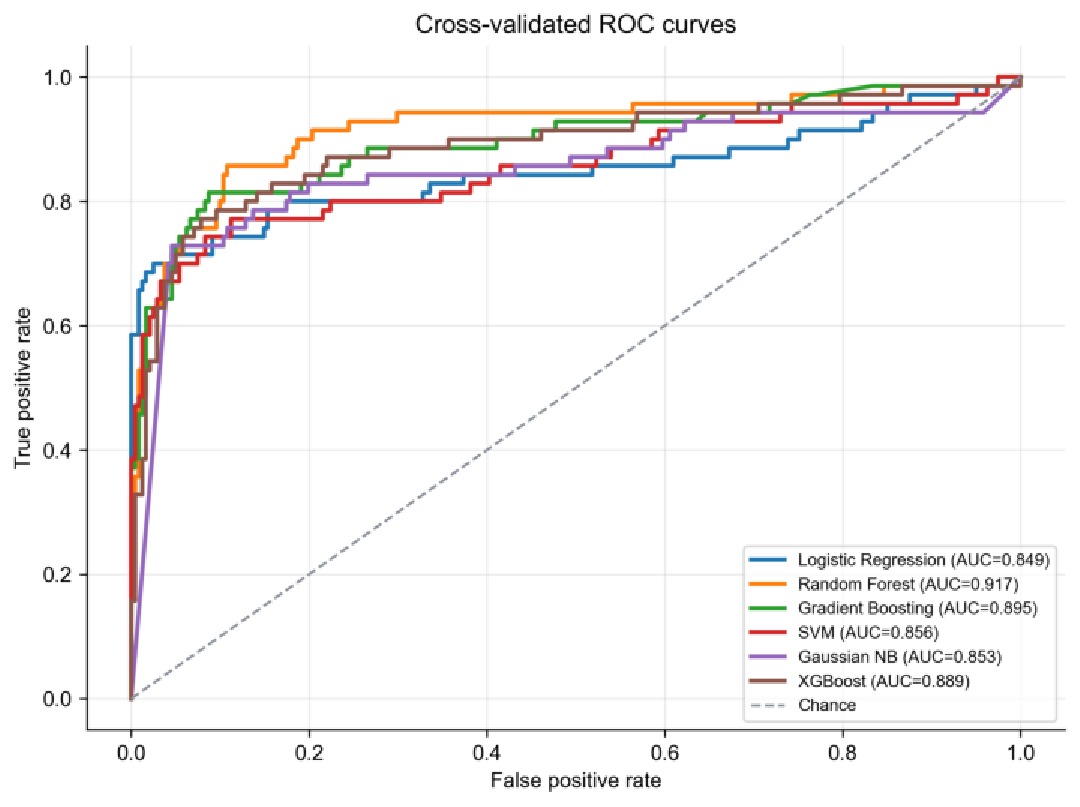
\includegraphics[width=0.78\linewidth]{figures/fig2_roc_curve.pdf}
\caption{Cross-validated ROC curves based on out-of-fold predictions.}
\label{fig:roc}
\end{figure}

\begin{figure}[H]
\centering
\begin{subfigure}{0.48\linewidth}
  \centering
  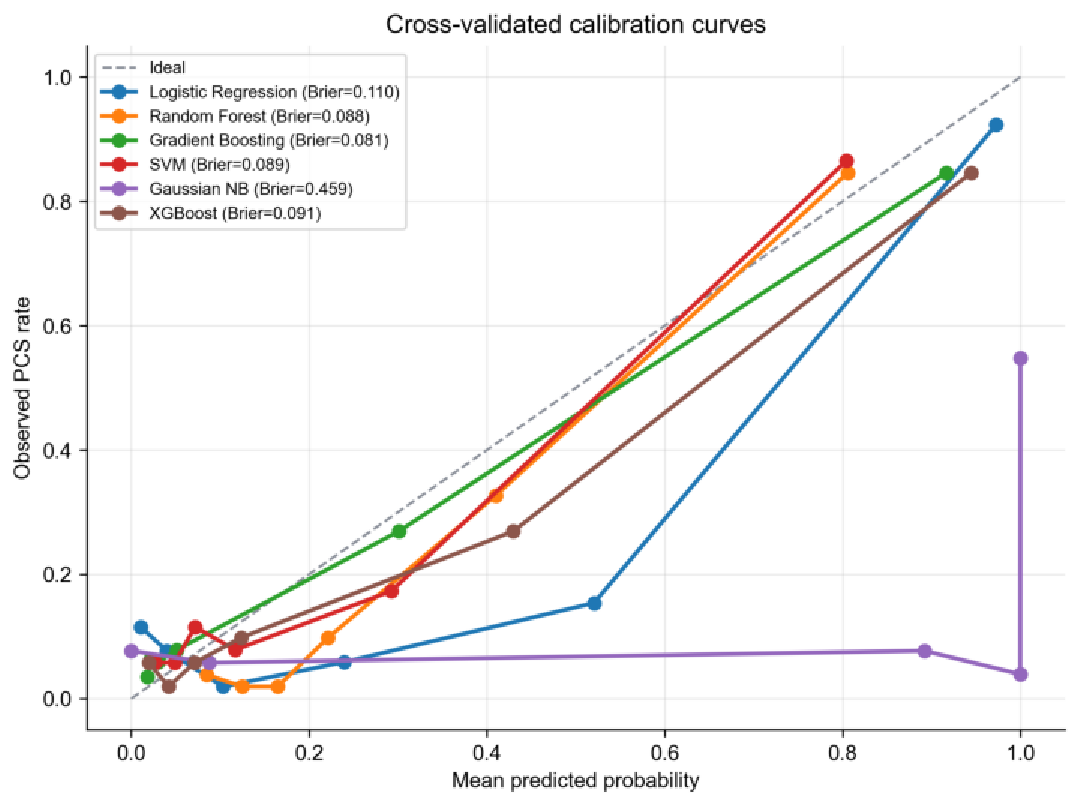
\includegraphics[width=\linewidth]{figures/fig3_calibration_curve.pdf}
  \caption{Calibration curves}
\end{subfigure}
\hfill
\begin{subfigure}{0.48\linewidth}
  \centering
  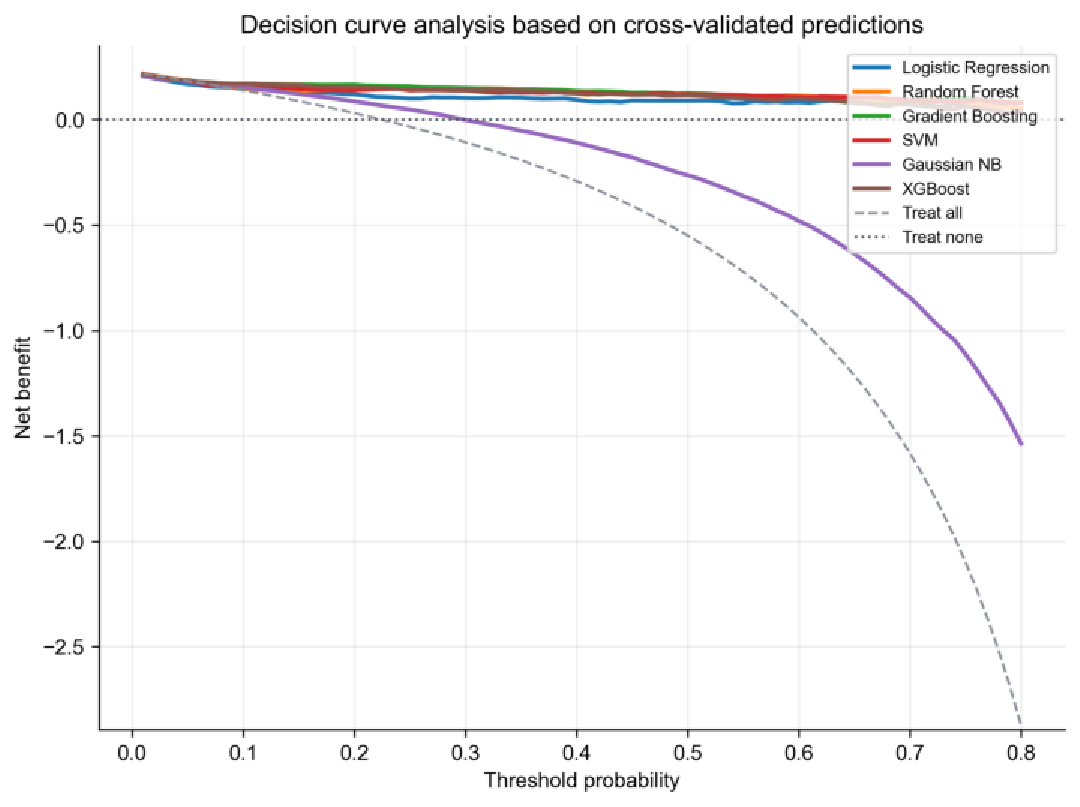
\includegraphics[width=\linewidth]{figures/fig4_dca_curve.pdf}
  \caption{Decision curve analysis}
\end{subfigure}
\caption{Clinical model assessment beyond discrimination.}
\label{fig:calibration_dca}
\end{figure}

\section{SHAP-Based Interpretation}

Random forest was selected for SHAP analysis because it achieved the best out-of-fold AUC. The fitted model mainly relied on hepatobiliary laboratory markers and symptom-related variables. The leading variables by aggregated mean absolute SHAP value were GGT, ALT, AST, ALP, CA19-9, total bilirubin, symptom duration, total bile acid, pain frequency, and age.

\begin{figure}[H]
\centering
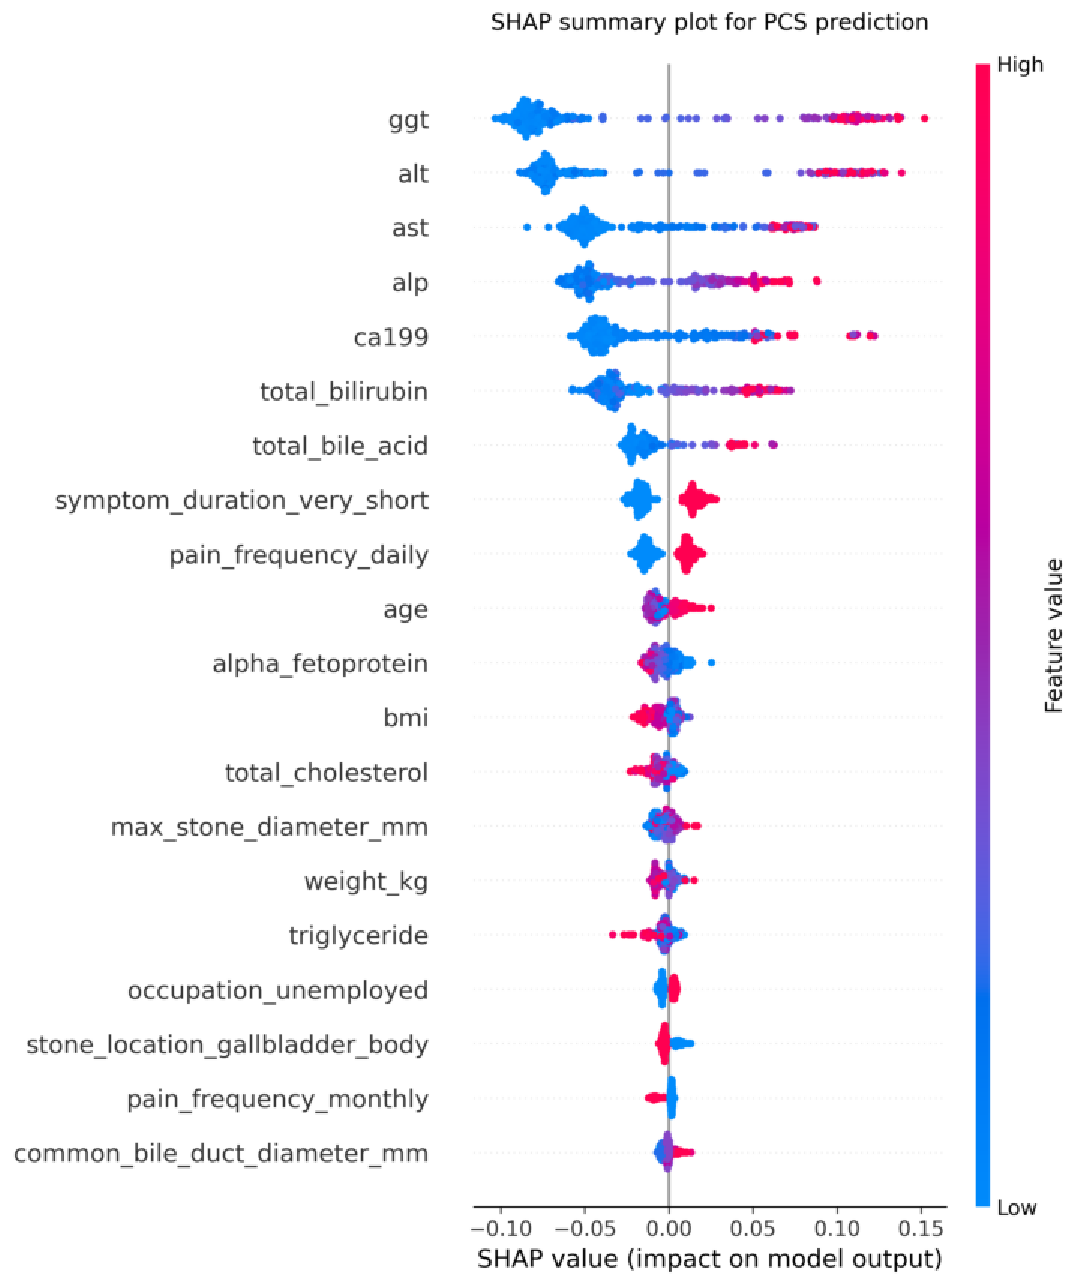
\includegraphics[width=0.85\linewidth]{figures/fig5_shap_summary.pdf}
\caption{SHAP summary plot for the final random forest model.}
\label{fig:shap_summary}
\end{figure}

\begin{figure}[H]
\centering
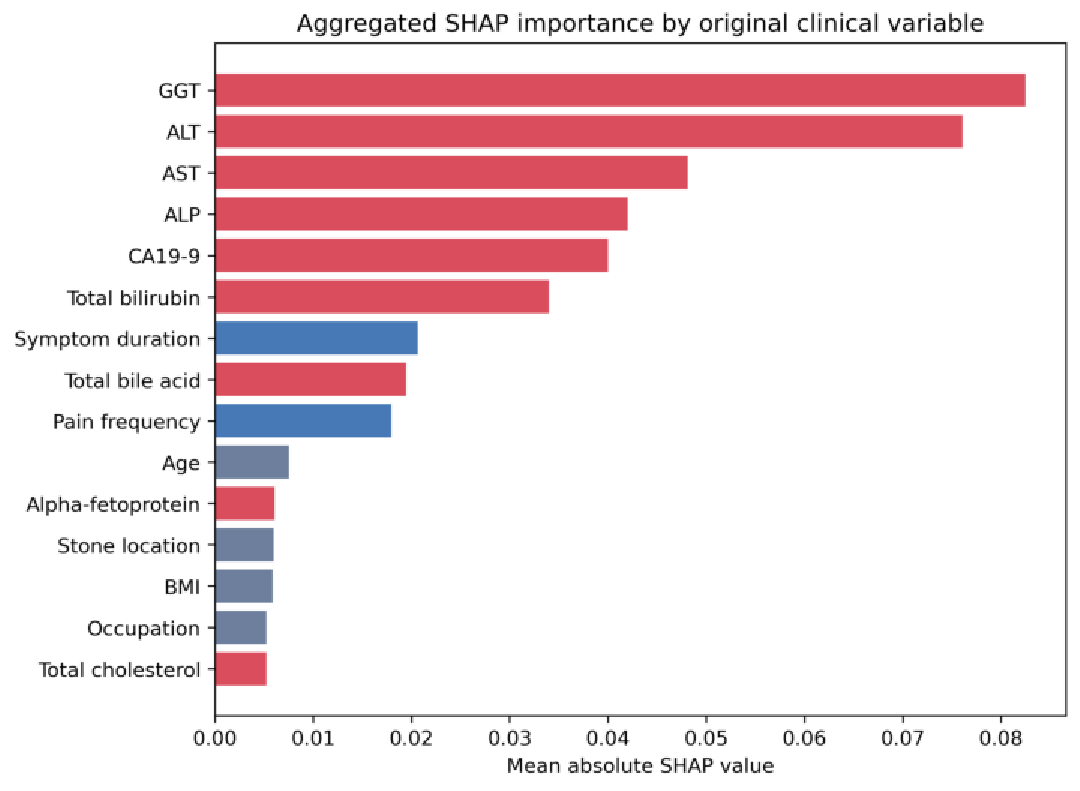
\includegraphics[width=0.75\linewidth]{figures/fig6_shap_variable_importance.pdf}
\caption{Aggregated SHAP importance by original clinical variable.}
\label{fig:shap_importance}
\end{figure}

\section{Exploratory PCS Symptom-Category Task}

The original free-text field for PCS symptom type was mapped into structured labels. This downstream task was restricted to PCS-positive patients with known symptom text. PCS-negative patients were not included in the symptom-subtype classifier. PCS-positive symptom text was grouped into pain, constipation, and dyspepsia-related phenotypes. Raw entries originally recorded as intestinal dysbiosis or gastrointestinal dysfunction were treated as dyspepsia symptoms for labeling, while the underlying mechanisms can be discussed separately. This task was treated as an exploratory secondary analysis because symptom subtype sample sizes were small.

\begin{table}[H]
\centering
\caption{Constructed PCS symptom occurrence categories in the full cohort.}
\label{tab:symptom_classes}
\small
\begin{tabular}{lcc}
\toprule
Category & Description & Count \\
\midrule
\texttt{no\_pcs} & No PCS & 241 \\
\texttt{pain} & Abdominal pain phenotype & 24 \\
\texttt{constipation} & Constipation phenotype & 19 \\
\texttt{gi\_dysfunction\_dyspepsia} & Dyspepsia-related phenotype & 26 \\
\texttt{pcs\_unknown} & PCS-positive with missing symptom text & 1 \\
\bottomrule
\end{tabular}
\end{table}

\begin{table}[H]
\centering
\caption{Exploratory downstream symptom-subtype prediction performance among PCS-positive patients.}
\label{tab:symptom_model_performance}
\small
\begin{tabular}{lcccc}
\toprule
Model & Accuracy & Balanced accuracy & Macro F1 & Macro OVR AUC \\
\midrule
XGBoost & 0.391 & 0.380 & 0.381 & 0.529 \\
Multinomial Logistic & 0.391 & 0.382 & 0.381 & 0.565 \\
Random Forest & 0.391 & 0.373 & 0.365 & 0.548 \\
Gradient Boosting & 0.362 & 0.351 & 0.348 & 0.544 \\
SVM & 0.246 & 0.225 & 0.197 & 0.445 \\
\bottomrule
\end{tabular}
\end{table}

\begin{figure}[H]
\centering
\begin{subfigure}{0.48\linewidth}
  \centering
  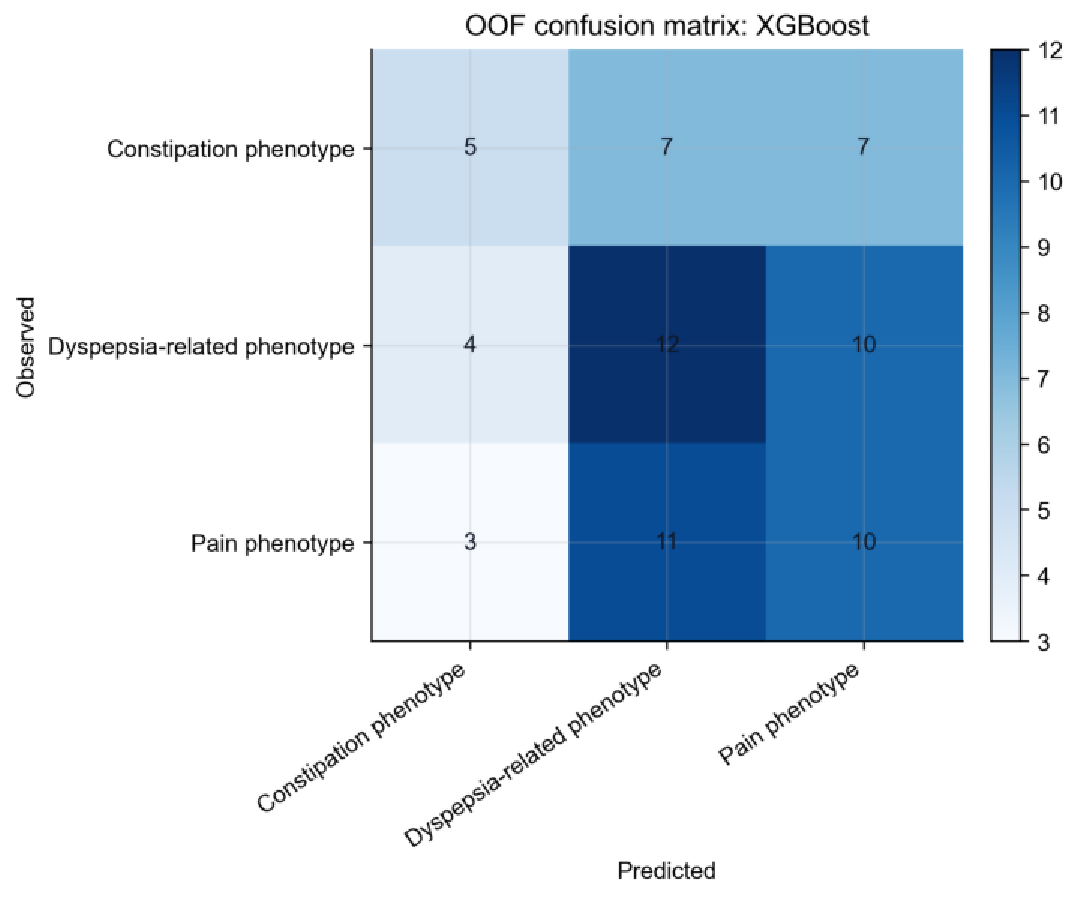
\includegraphics[width=\linewidth]{figures/figS2_symptom_confusion_matrix.pdf}
  \caption{Confusion matrix}
\end{subfigure}
\hfill
\begin{subfigure}{0.48\linewidth}
  \centering
  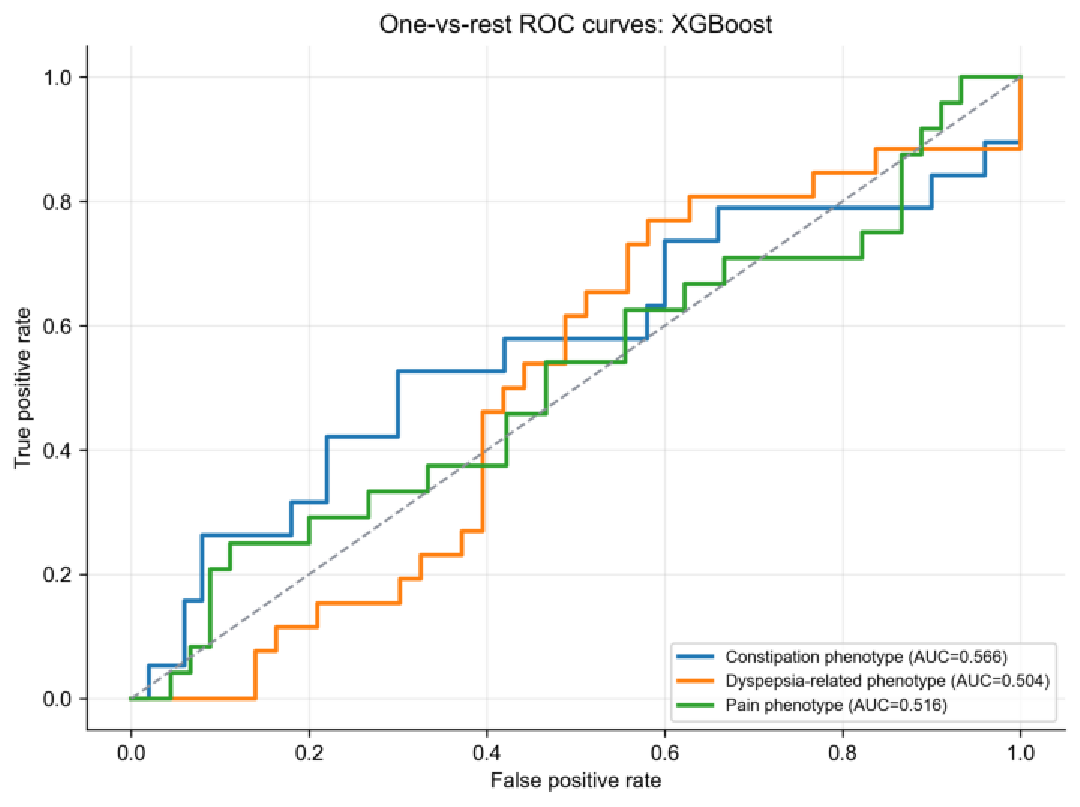
\includegraphics[width=\linewidth]{figures/figS3_symptom_ovr_roc.pdf}
  \caption{One-vs-rest ROC}
\end{subfigure}
\caption{Exploratory downstream PCS symptom-subtype prediction results. Balanced accuracy is calculated only across PCS symptom subtypes and excludes \texttt{no\_pcs}.}
\label{fig:symptom_task}
\end{figure}

\section{Exploratory Latent Phenotype Analysis}

Unsupervised dimensionality reduction and clustering were used to explore whether the preoperative feature space contained latent phenotypes related to PCS occurrence or symptom subtypes. This analysis was exploratory and hypothesis-generating. K-means selected a two-cluster solution based on the highest silhouette score. Cluster 0 showed a markedly higher PCS rate than cluster 1.

\begin{table}[H]
\centering
\caption{Latent cluster summary.}
\label{tab:cluster_summary}
\small
\begin{tabular}{lcccc}
\toprule
Cluster & N & PCS cases & PCS rate & Median PCS onset, days \\
\midrule
0 & 45 & 43 & 95.6\% & 43.0 \\
1 & 266 & 27 & 10.2\% & 86.0 \\
\bottomrule
\end{tabular}
\end{table}

\begin{figure}[H]
\centering
\begin{subfigure}{0.48\linewidth}
  \centering
  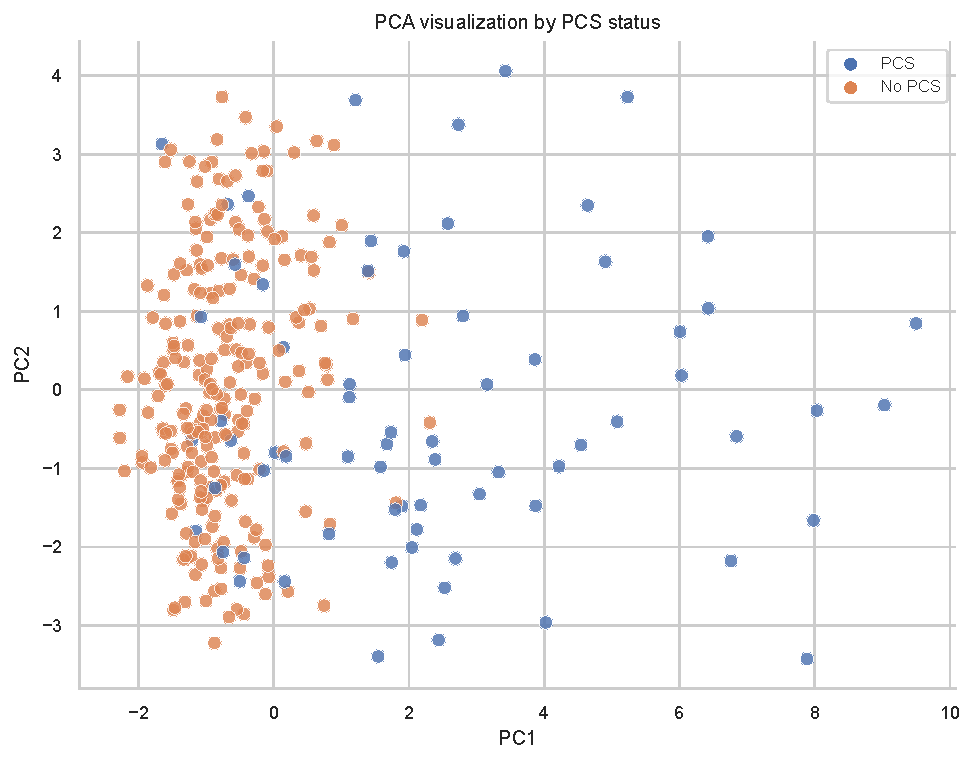
\includegraphics[width=\linewidth]{figures/figS4_pca_by_pcs.pdf}
  \caption{PCA by PCS status}
\end{subfigure}
\hfill
\begin{subfigure}{0.48\linewidth}
  \centering
  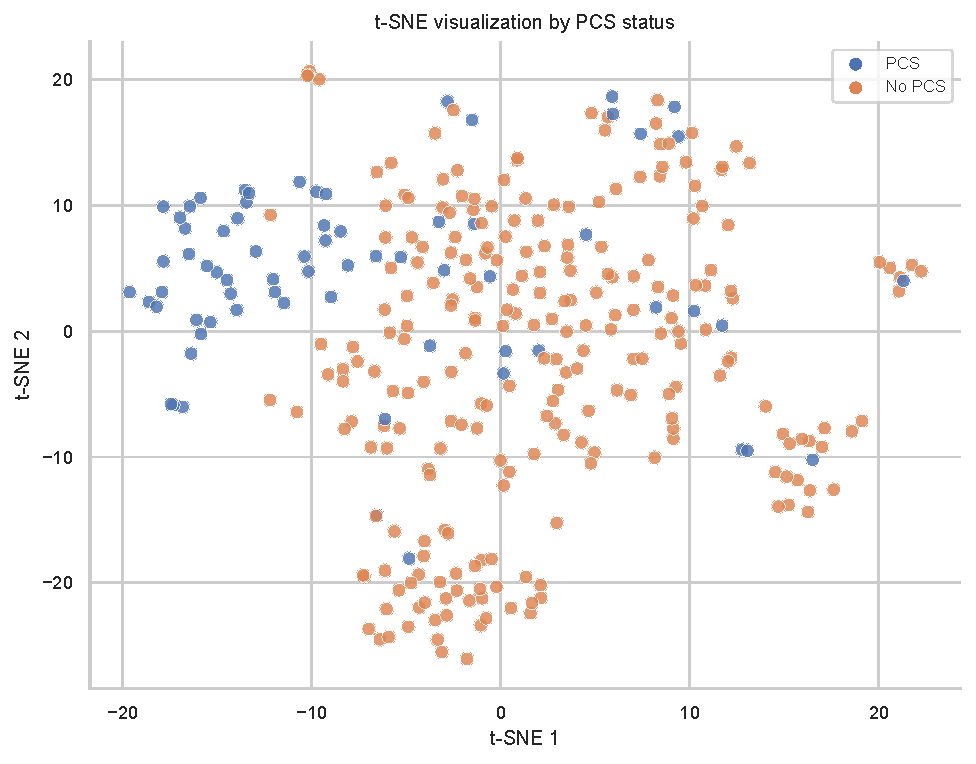
\includegraphics[width=\linewidth]{figures/figS4_tsne_by_pcs.pdf}
  \caption{t-SNE by PCS status}
\end{subfigure}
\caption{Exploratory dimensionality reduction using preoperative variables.}
\label{fig:latent_embedding}
\end{figure}

\begin{figure}[H]
\centering
\begin{subfigure}{0.48\linewidth}
  \centering
  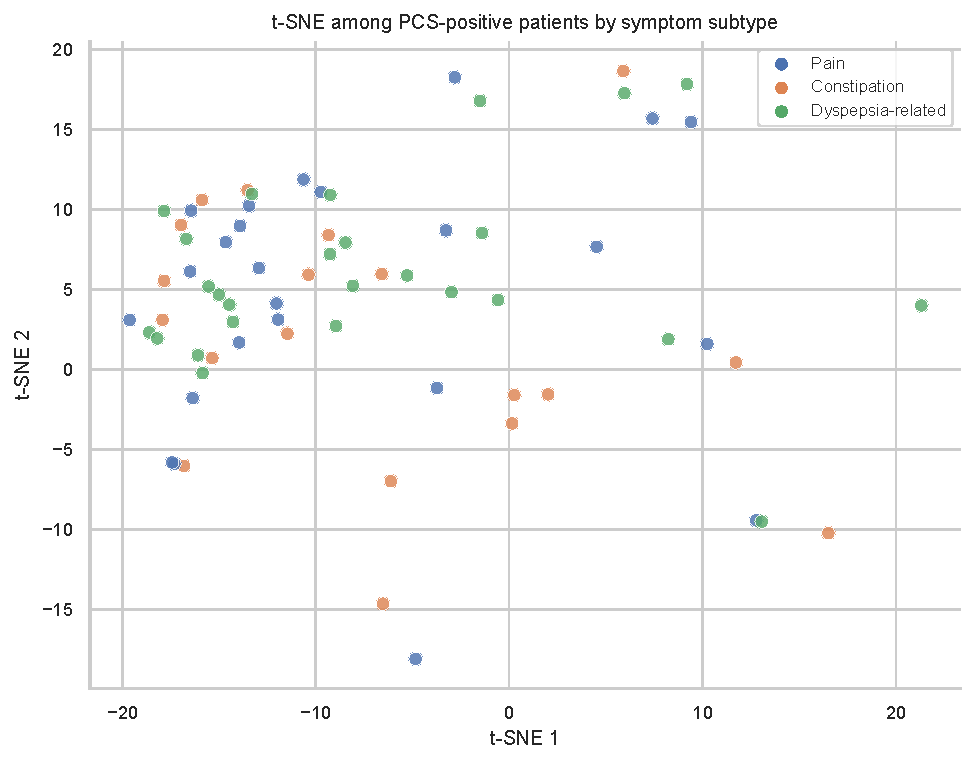
\includegraphics[width=\linewidth]{figures/figS4_tsne_pcs_positive_by_symptom.pdf}
  \caption{PCS-positive patients by symptom subtype}
\end{subfigure}
\hfill
\begin{subfigure}{0.48\linewidth}
  \centering
  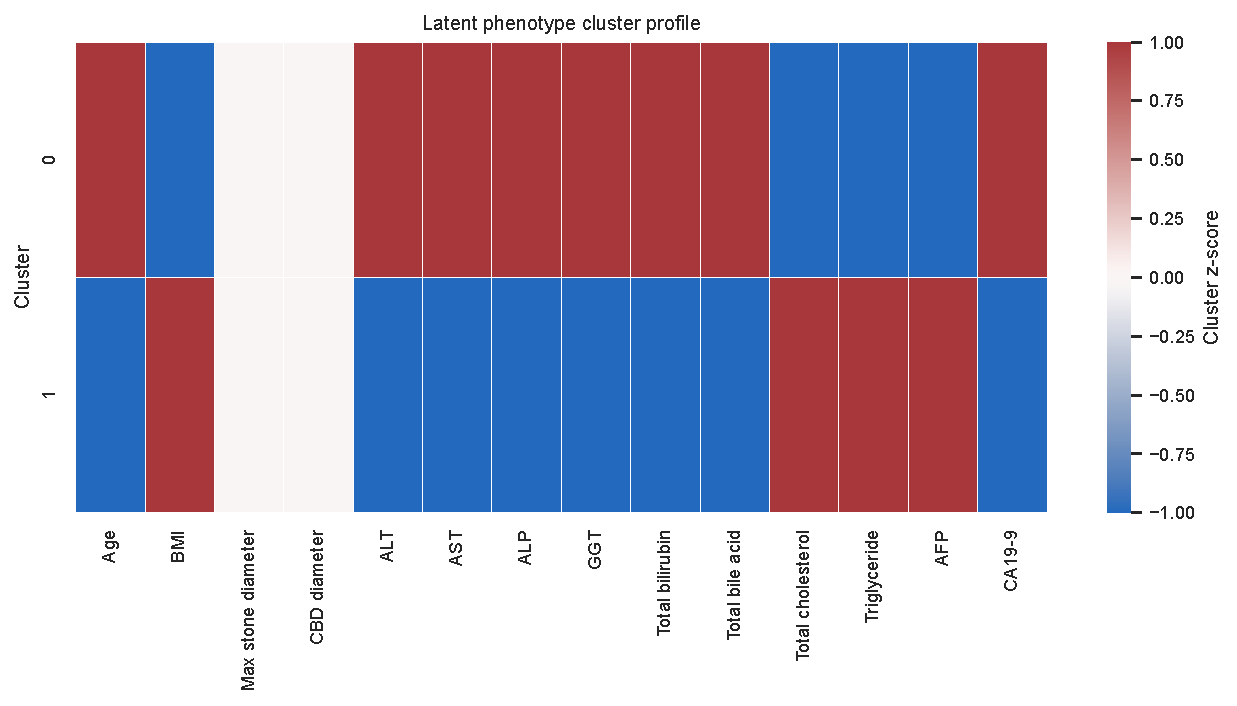
\includegraphics[width=\linewidth]{figures/figS5_cluster_heatmap.pdf}
  \caption{Cluster feature profile}
\end{subfigure}
\caption{Exploratory latent phenotype structure.}
\label{fig:latent_symptom_cluster}
\end{figure}

\begin{figure}[H]
\centering
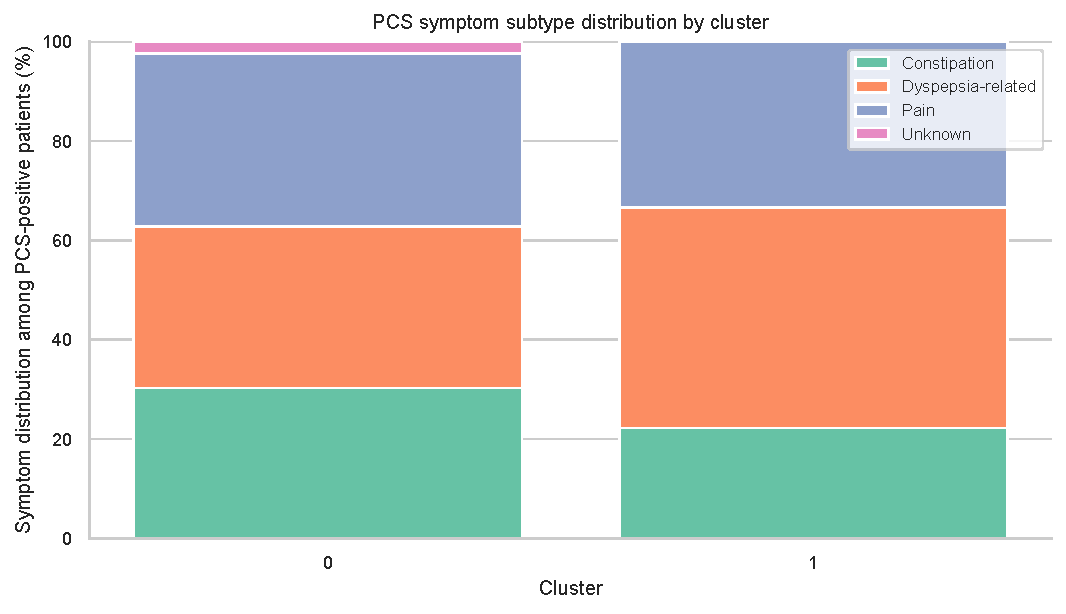
\includegraphics[width=0.72\linewidth]{figures/figS7_cluster_symptom_distribution.pdf}
\caption{PCS symptom subtype distribution by latent cluster. Cluster-level PCS rates are reported in Table~\ref{tab:cluster_summary}.}
\label{fig:latent_cluster_outcomes}
\end{figure}

\section{Current Interpretation}

The current results suggest that machine-learning models can provide strong internal discrimination for PCS occurrence, with random forest achieving the best out-of-fold AUC. SHAP analysis indicated that laboratory markers of hepatobiliary disturbance contributed most prominently to model predictions. The symptom-category task provides an initial framework for modeling PCS heterogeneity, but the class sizes are limited and the results should be interpreted as exploratory.

\section{Limitations}

This demo uses internal cross-validation only. External validation, prospective assessment, formal hyperparameter tuning, complete baseline regression analysis, and clinically defined risk thresholds remain necessary before clinical deployment.

\end{document}
